
\documentclass[a4paper,12pt]{article}
%%%%%%%%%%%%%%%%%%%%%%%%%%%%%%%%%%%%%%%%%%%%%%%%%%%%%%%%%%%%%%%%%%%%%%%%%%%%%%%%%%%%%%%%%%%%%%%%%%%%%%%%%%%%%%%%%%%%%%%%%%%%%%%%%%%%%%%%%%%%%%%%%%%%%%%%%%%%%%%%%%%%%%%%%%%%%%%%%%%%%%%%%%%%%%%%%%%%%%%%%%%%%%%%%%%%%%%%%%%%%%%%%%%%%%%%%%%%%%%%%%%%%%%%%%%%
\usepackage{eurosym}
\usepackage{vmargin}
\usepackage{amsmath}
\usepackage{graphics}
\usepackage{epsfig}
\usepackage{subfigure}
\usepackage{fancyhdr}
\usepackage{listings}
\usepackage{framed}
\usepackage{graphicx}

\setcounter{MaxMatrixCols}{10}
%TCIDATA{OutputFilter=LATEX.DLL}
%TCIDATA{Version=5.00.0.2570}
%TCIDATA{<META NAME="SaveForMode" CONTENT="1">}
%TCIDATA{LastRevised=Wednesday, February 23, 2011 13:24:34}
%TCIDATA{<META NAME="GraphicsSave" CONTENT="32">}
%TCIDATA{Language=American English}

\pagestyle{fancy}
\setmarginsrb{20mm}{0mm}{20mm}{25mm}{12mm}{11mm}{0mm}{11mm}
\lhead{MA4128} \rhead{Mr. Kevin O'Brien}
\chead{Principal Component Analysis}
%\input{tcilatex}

\begin{document}
	
	
	\subsection{Determining the Number of “Meaningful” Components to Retain}
	Earlier it was stated that the number of components extracted is equal to the number of variables
	being analyzed, necessitating that you decide just how many of these components are truly
	meaningful and worthy of being retained for further analysis.
	
	In general, you expect
	that only the first few components will account for meaningful amounts of variance, and that the
	later components will tend to account for only trivial variance.
	
	The next step of the analysis,therefore, is to determine how many meaningful components should be retained for
	interpretation.  The followings section will describe four criteria that may be used in making this decision:
	\begin{itemize} \item the eigenvalue-one criterion, \item the scree test, \item the proportion of variance accounted for, \item the
		interpretability criterion.
	\end{itemize}
	
	
	\subsection{The Eigenvalue-One Criterion}  In principal component analysis, one of the most commonly
	used criteria for solving the number-of-components problem is the eigenvalue-one criterion, also
	known as the Kaiser criterion (Kaiser, 1960).  With this approach, you retain and interpret any
	component with an eigenvalue greater than 1.00.
	
	The rationale for this criterion is straightforward.  Each observed variable contributes one unit of
	variance to the total variance in the data set.  Any component that displays an eigenvalue greater
	than 1.00 is accounting  for a greater amount of variance than had been contributed by one
	variable.  Such a component is therefore accounting for a meaningful amount of variance, and is
	worthy of being retained.
	
	On the other hand, a component with an eigenvalue less than 1.00 is accounting for less variance
	than had been contributed by one variable.  The purpose of principal component analysis is to
	reduce a number of observed variables into a relatively smaller number of components; this
	cannot be effectively achieved if you retain components that account for less variance than had
	been contributed by individual variables.  For this reason, components with eigenvalues less than
	1.00 are viewed as trivial, and are not retained.
	
	
	\subsubsection{Advantages and Disadvantages}
	The eigenvalue-one criterion has a number of positive features that have contributed to its
	popularity.  Perhaps the most important reason for its widespread use is its simplicity:  You do
	not make any subjective decisions, but merely retain components with eigenvalues greater than
	one.
	
	On the positive side, it has been shown that this criterion very often results in retaining the
	correct number of components, particularly when a small to moderate number of variables are
	being analyzed and the variable communalities are high.  Stevens (1986) reviews studies that
	have investigated the accuracy of the eigenvalue-one criterion, and recommends its use when
	less than 30 variables are being analyzed and communalities are greater than .70, or when the
	analysis is based on over 250 observations and the mean communality is greater than or equal to
	0.60.
	
	There are a number of problems associated with the eigenvalue-one criterion, however.  As was
	suggested in the preceding paragraph, it can lead to retaining the wrong number of components
	under circumstances that are often encountered in research (e.g., when many variables are
	analyzed, when communalities are small).
	
	Also, the mindless application of this criterion can
	lead to retaining a certain number of components when the actual difference in the eigenvalues
	of successive components is only trivial.  For example, if component 2 displays an eigenvalue of
	1.001 and component 3 displays an eigenvalue of 0.999, then component 2 will be retained but
	component 3 will not; this may mislead you into believing that the third component was
	meaningless when, in fact, it accounted for almost exactly the same amount of variance as the
	second component.
	
	In short, the eigenvalue-one criterion can be helpful when used judiciously,
	but the thoughtless application of this approach can lead to serious errors of interpretation.
	
	\subsection{The scree test} With the scree test (Cattell, 1966), you plot the eigenvalues associated with
	each component and look for a “break” between the components with relatively large
	eigenvalues and those with small eigenvalues.  The components that appear before the break are
	assumed to be meaningful and are retained for rotation; those apppearing after the break are
	assumed to be unimportant and are not retained.
	
	Remark: The word “scree” refers to the loose rubble that lies at
	the base of a cliff.  When performing a scree test, you normally hope that the scree plot
	will take the form of a cliff:  At the top will be the eigenvalues for the few meaningful
	components, followed by a break (the edge of the cliff).  At the bottom of the cliff will lie
	the scree:  eigenvalues for the trivial components.
	
	\begin{figure}[h!]
		\begin{center}
			% Requires \usepackage{graphicx}
			\includegraphics[scale=0.9]{3AScree1.jpg}\\
			\caption{Example of a Scree Plot}\label{Scree Plot}
		\end{center}
		
	\end{figure}
	
	
	Sometimes a scree plot will display several large breaks.  When this is the case, you should look
	for the last big break before the eigenvalues begin to level off. Only the components that appear
	before this last large break should be retained.
	
	\subsubsection{Advantages and Disadvantages}
	The scree test can be expected to provide reasonably accurate results, provided the sample is
	large (over 200) and most of the variable communalities are large (Stevens, 1986).  However,
	this criterion has its own weaknesses as well, most notably the ambiguity that is often displayed
	by scree plots under typical research conditions:  Very often, it is difficult to determine exactly
	where in the scree plot a break exists, or even if a break exists at all.
	
	\subsection{Proportion of Variance Accounted For}
	
	A third criterion in solving the number of factors
	problem involves retaining a component if it accounts for a specified proportion (or percentage)
	of variance in the data set.  For example, you may decide to retain any component that accounts
	for at least $5\%$ or $10\%$ of the total variance.  This proportion can be calculated with a simple
	formula:
	
	\[ \mbox{Proportion}  = \frac{\mbox{Eigenvalue for the component of interest}}{\mbox{Total eigenvalues of the correlation matrix}}  \]
	
	In principal component analysis, the “total eigenvalues of the correlation matrix” is equal to the
	total number of variables being analyzed (because each variable contributes one unit of variance
	to the analysis).
	
	An alternative criterion is to retain enough components so that the cumulative percent of variance
	accounted for is equal to some minimal value.  Suppose that,in a PCA procedure, that components 1, 2, 3,
	and 4 accounted for approximately $37\%$, $33\%$, $13\%$, and $10\%$ of the total variance, respectively.
	
	Suppose that it was required to account for $90\%$ of the variance. Adding these percentages together results in a sum of $93\%$.  This means that the cumulative percent of variance accounted for by components 1, 2, 3, and 4 is $93\%$.
	
	\begin{figure}[h!]
		\begin{center}
			% Requires \usepackage{graphicx}
			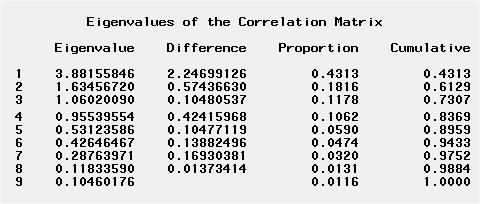
\includegraphics[scale=0.9]{3AEigen.jpg}\\
			\caption{Eigenvalue Table}\label{Eigenvalue Table}
		\end{center}
		
	\end{figure}
	
	
	\subsubsection{Advantages and Disadvantages}
	
	The proportion of variance criterion has a number of positive features.  For example, in most
	cases, you would not want to retain a group of components that, combined, account for only a
	minority of the variance in the data set (say, $30\%$).  Nonetheless, many critical values discussed
	earlier are obviously arbitrary.  Because of these and related problems, this approach has sometimes been
	criticized for its subjectivity (Kim and Mueller, 1978).
	
	\subsection{The Interpretability Criteria}
	
	Perhaps the most important criterion for solving the \textbf{\emph{number of-components}} problem is the interpretability criterion:  interpreting the substantive meaning of the retained components and verifying that this interpretation makes sense in terms of what is known about the constructs under investigation.
	
	
	The following list provides four rules to follow in doing this.  (A later section shows how to
	actually interpret the results of a principal component analysis; the following rules will be more
	meaningful after you have completed that section).
	
	\begin{enumerate}
		\item Are there at least three variables (items) with significant loadings on each retained
		component?  A solution is less satisfactory if a given component is measured by less than
		three variables.
		
		\item  Do the variables that load on a given component share the same conceptual meaning?
		For example, if three questions on a survey all load on component 1, do all three of these
		questions seem to be measuring the same construct?
		
		\item  Do the variables that load on different components seem to be measuring different
		constructs?  For example, if three questions load on component 1, and three other
		questions load on component 2, do the first three questions seem to be measuring a
		construct that is conceptually different from the construct measured by the last three
		questions?
		
		\item  Does the rotated factor pattern demonstrate “simple structure?”  Simple structure
		means that the pattern possesses two characteristic:
		
		\begin{itemize}
			\item[(a)] Most of the variables have
			relatively high factor loadings on only one component, and near zero loadings on the other
			components, and \item[(b)] most components have relatively high factor loadings for some
			variables, and near-zero loadings for the remaining variables.
		\end{itemize}
	\end{enumerate}
	\newpage
\end{document}	